\chapter{Apache Kafka in caso d’uso simulato}

\section{Definizione di un \textit{way of working}}

% Descrizione del Piano di Lavoro presentato, le strategie e il metodo di lavoro stabilito.
All'inizio del percorso ho delineato un \textit{way of working}, ovvero un metodo di lavoro da mantenere per tutta la durata dello \textit{stage}, insieme al tutor aziendale, il responsabile del settore \sacr{eai} e gli esperti del settore.

Per mantenere un buon livello organizzativo, quantificare l'avanzamento e rendere agevole la verifica e il supporto tecnico l'azienda ha proposto l'utilizzo di una \textit{board} di progetto.
Tra le tante opzioni disponibili, mi è stata proposta la piattaforma \textit{ClickUp}.
Rispetto alla concorrenza questa \textit{board} è ricca di funzionalità, pulita nell'esposizione dello stato del progetto, e la maggior parte delle sue funzioni sono gratuite.

All'inizio del percorso il tutor aziendale e il responsabile del \sacr{eai} hanno creato delle \textit{card} contenenti le attività previste per ogni settimana (\textit{task}) al fine di fornire una struttura generale del progetto.
All'interno di questi \textit{task} vi sono i concetti chiave, attività previste e obiettivi settimanali che lo stagista è tenuto a seguire per garantire l'efficacia del prodotto finale.
Oltre a questi \textit{task} principali, ho potuto creare di \textit{task} ausiliari e dei \textit{subtask} per descrivere più adeguatamente l'attività in corso.

Ciascun \textit{task} contiene una colonna laterale dove ho mantenuto un \textit{log} di tutto ciò che è stato eseguito relativo al \textit{task} in questione, allo scopo di esplicitarne il progresso e rendere agevole un eventuale supporto dal tutor o l'evoluzione futura.

Ogni settimana è previsto un \textit{online meeting} per la verifica del progresso ove necessario, la risposta ad eventuali questioni sollevate, e spiegazioni riguardo lo sviluppo della settimana successiva.
Alcune di queste videoconferenze ha visto la partecipazione di altri esperti che mi hanno aiutato a comprendere meglio il caso d'uso da reingegnerizzare, riassumendo lo stato attuale del sistema d'integrazione per uno dei clienti con relativi \textit{file} utilizzati.

Per mantenere alto il livello di organizzazione, efficienza ed efficacia, all'inizio di ogni giornata lavorativa ho creato un breve piano giornaliero con successivo consuntivo a fine giornata.
Questo ha permesso al tutor di verificare rapidamente il corretto avanzamento del processo in corso e a me di mantenere il \textit{focus} su di esso.

\section{Formazione}

Il processo di Formazione ha avuto un importante ruolo all'interno dello \textit{stage}, con una durata complessiva di circa quattro settimane.
La causa di questo lungo periodo è data dallo studio di diversi ambiti e concetti, in particolare il settore del \textit{\acrlong{eai}} e la nuova tecnologia di Kafka.

Durante questo processo Sync Lab mi ha fornito del materiale didattico per l'apprendimento, quali diapositive e appunti di origine aziendale e l'accesso a dei corsi riguardo \textit{Software architecture}, \textit{\acrlong{soa}} (tramite i corsi online su \textit{Coursera}) e Apache Kafka (tramite i corsi online su \textit{Udemy}).

Il tutor aziendale e responsabile \sacr{eai} hanno fornito durante i \textit{meeting} settimanali ulteriori chiarimenti e approfondimenti sul come Sync Lab applica questi concetti nello sviluppo di architetture \software.

Per i corsi online a maggiore contenuto nozionistico ho redatto degli appunti riassuntivi, con lo scopo di consolidare l'apprendimento e velocizzare la verifica del tutor aziendale.

\section{Progettazione di un caso d'uso}

Ad alcune videoconferenze ha partecipato anche un altro esperto \textit{senior} aziendale, esterno al progetto di \stage\ in questione, per illustrarmi un caso d'uso in cui l'azienda ha esposto un prototipo di sistema di integrazione utilizzando i concetti di \textit{Web Service}, \sacrfoot{soap} e \textit{request/response}, permettendomi la visualizzazione dei file \sacrfoot{wsdl}, \sacrfoot{xml} e \sacrfoot{xsd} associati.
Ho pertanto generato un caso d'uso adatto agli scopi dello \stage\ ispirandomi al caso d'uso reale illustrato.

Il caso d'uso modellato tratta una richiesta di credito telefonico da parte di un cliente ad un'azienda di telecomunicazioni tramite \textit{Web Service}, per soddisfare il requisito dello sviluppo della reingegnerizzazione del flusso di dati asincrono.
La \textit{request} avviene tramite flusso di un file \sacrfoot{json} che viene trasmesso attraverso i vari servizi che compongono il sistema di integrazione, basatosul \textit{Design Pattern} di tipo \textit{publish/subscribe}.

Va precisato che il contenuto di tale \sacr{json} non è strettamente rilevante allo sviluppo e funzionamento del \textit{Middleware}, ma aiuta a stabilire il contesto di utilizzo.

\bigskip
\begin{figure}[h]
  \begin{center}
    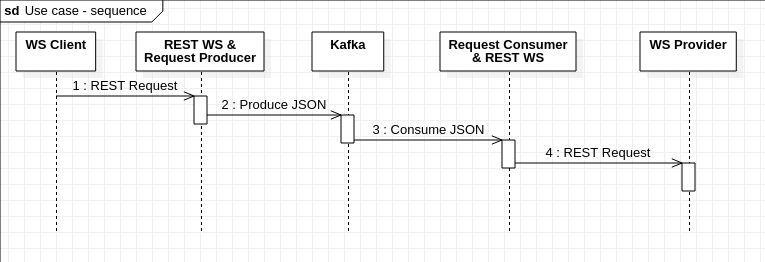
\includegraphics[width=\textwidth, trim={0.08cm 0 0 0.08cm},clip]{images/uc_sequence.png}
    \caption{Diagramma di sequenza \sacr{uml} per il prototipo di caso d'uso iniziale}
    \captionsetup{aboveskip=2pt}
    \caption*{\begin{footnotesize}\textit{Fonte: elaborazione personale}\end{footnotesize}}
  \end{center}
\end{figure}

\noindent
Il caso d'uso (figura \thefigure) è composto dai seguenti passaggi:
\begin{enumerate}
  \item il cliente (\textit{\sacrfoot{ws} Client}) effettua una richiesta di credito tramite invio di un file \sacr{json} al successivo Servizio Web in ascolto.
  \item il servizio composto da \sacrfoot{rest} \sacr{ws} e \textit{Request Producer} riceve il \sacr{json} e lo inserisce in Kafka tramite l'apposito \textit{Kafka Producer}, assumendo la funzione di \textit{publisher}.
  \item il servizio di \textit{Request Consumer}, sottoscritto al \textit{topic} in questione riceve il \sacr{json} e lo invia al \sacr{ws} finale tramite una \sacr{rest} request.
  \item il servizio in coda chiamato \sacr{ws} \textit{Provider} riceve il \sacr{json}; grazie ai dati ricevuti è in grado di fornire il servizio richiesto dal \textit{Client} nello \textit{step} 1.
\end{enumerate}

La modellazione dell'architetture e struttura del sistema da sviluppare seguirà questo prototipo di \sacrfoot{uc}.
Il modello associato al caso asincrono con \textit{callback} seguirà la stessa struttura e \textit{step} dello \sacr{uc} illustrato qui sopra, con l'aggiunta speculare del messaggio di ritorno.

\section{Progettazione architetturale}

La progettazione architetturale ha portato alla produzione di diversi diagrammi \sacr{uml} per rappresentare efficacemente l'architettura del prodotto e fornire un modello da seguire durante il processo di sviluppo.
Il processo ha richiesto frequenti \textit{meeting} e confronti per raggiungere un risultato finale soddisfacente al fine della sperimentazione.
% I diagrammi di maggiore rilevanza, oltre ad essere esposti all'interno di questa sezione accanto alla spiegazione associata, sono allegati in formato più grande a
I diagrammi rappresentano i componenti \textit{color coded}, notazione utilizzata per dare continuità e chiarezza attraverso le diverse tipologie di \sacr{uml} \textit{diagrams}.

\subsubsection{\sacr{uml} \textit{sequence diagrams}}


A partire dallo \sacr{uc} descritto nela sezione precedente, ho prodotto un \sacr{uml} \textit{sequence diagram} più approfondito per rappresentare il flusso del \sacr{json} tra i vari componenti (figura seguente).
\bigskip
\begin{figure}[h]
  \begin{center}
    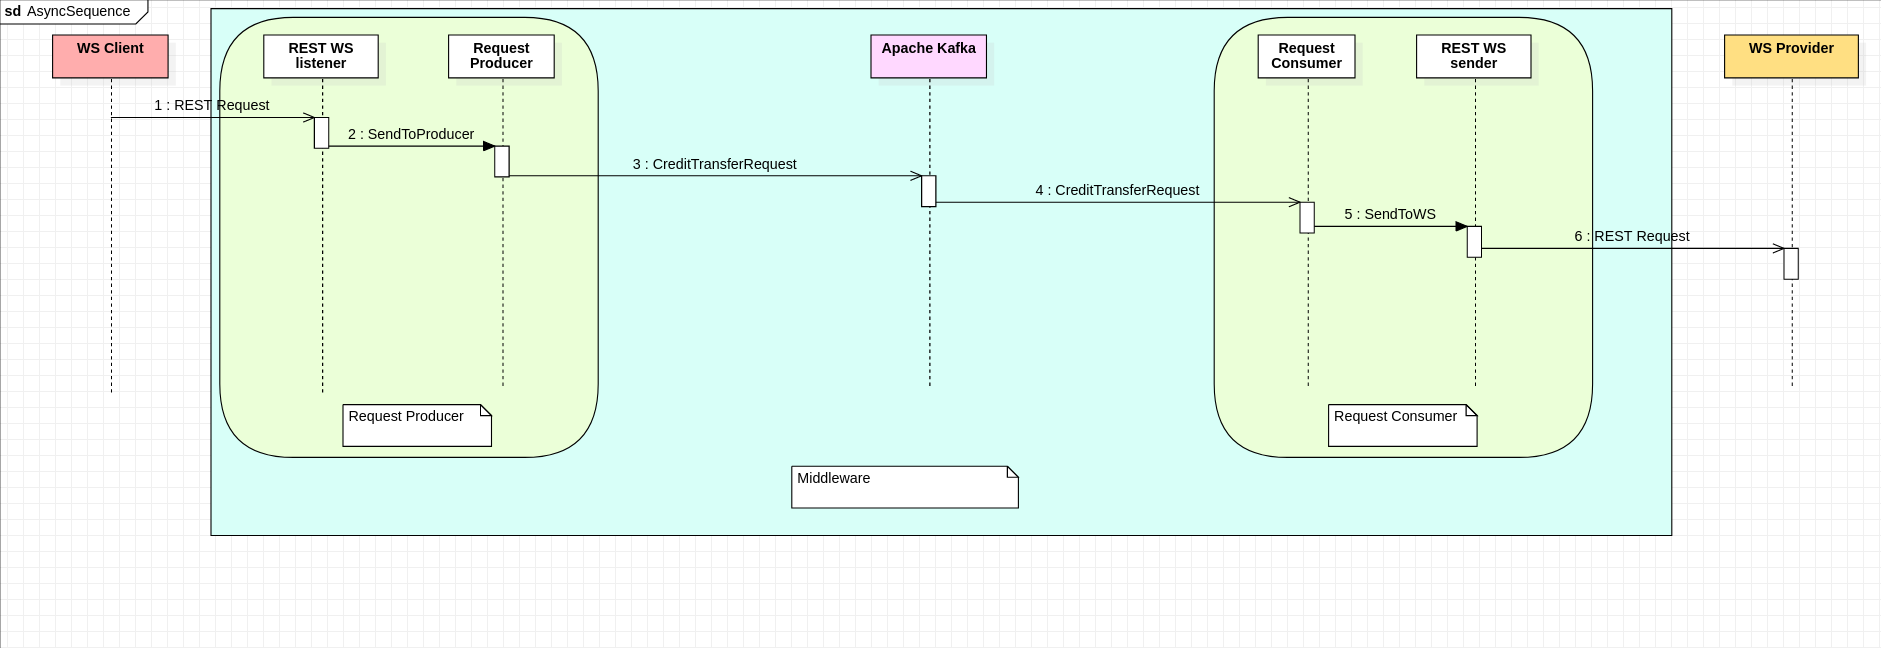
\includegraphics[width=\textwidth, trim={0.2cm 0 0 0.2cm},clip]{images/a_sequence2.png}
    \caption{Diagramma \sacr{uml} di sequenza per la reingegnerizzazione del flusso asincrono}
    \captionsetup{aboveskip=2pt}
    \caption*{\begin{footnotesize}\textit{Fonte: elaborazione personale}\end{footnotesize}}
  \end{center}
\end{figure}

La progettazione del sistema associato al caso asincrono con \textit{callback} comprende il flusso descritto qui sopra, con aggiunta del flusso di ritorno descritto nella figura seguente.
\bigskip
\begin{figure}[h]
  \begin{center}
    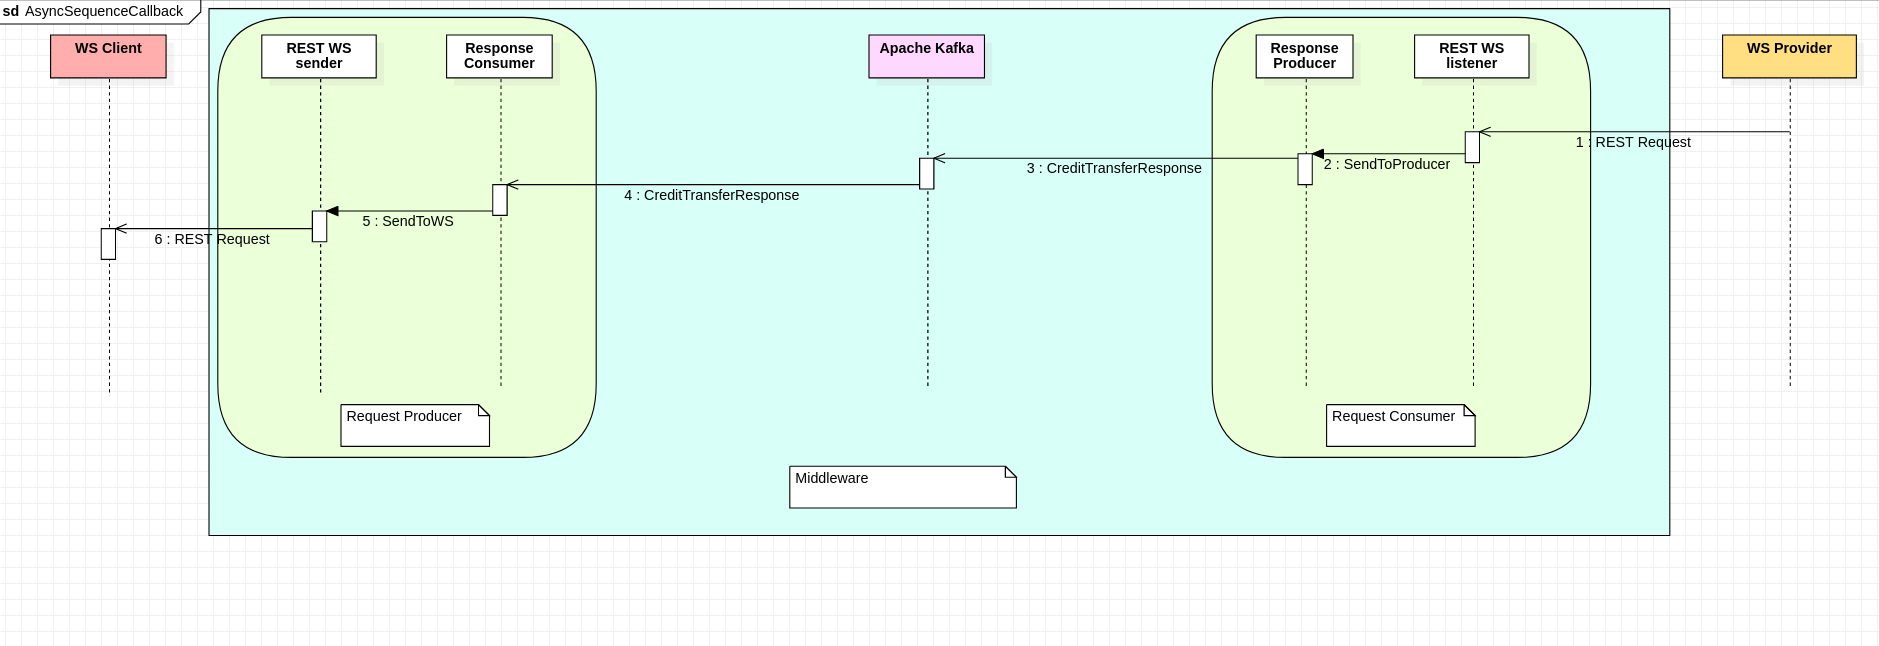
\includegraphics[width=\textwidth]{images/ac_sequence.png}
    \caption{Diagramma di sequenza \sacr{uml} per la reingegnerizzazione del flusso asincrono con \textit{callback}}
    \captionsetup{aboveskip=2pt}
    \caption*{\begin{footnotesize}\textit{Fonte: elaborazione personale}\end{footnotesize}}
  \end{center}
\end{figure}

La reingegnerizzazione del flusso sincrono è stata scartata in favore dello studio di funzionalità aggiuntive tramite l'utilizzo della piattaforma di \textit{event streaming}.
La progettazione di un sistema basato su questo flusso era inizialmente prevista (come requisito desiderabile) nel piano di lavoro iniziale poiché associata ad un caso d'uso reale (di cui si è parlato nelle sezioni precedenti), ma infine è stata giudicata poco opportuna e fuori dagli scopi di Apache Kafka, un sistema basato sull'asincronicità

Il tempo associato a tale requisito è stato pertanto riproposto per testare un'altra funzione utile in un \middleware\, quali la trasformazione di alcuni dati presenti nel \sacr{json}.
Più precisamente, è stato aggiunto un dato sensibile che viene nascosto e sostituito con asterischi "*" dopo la produzione del \textit{topic} in Kafka grazie all'utilizzo di Kafka Streams.
\bigskip
\begin{figure}[h]
  \begin{center}
    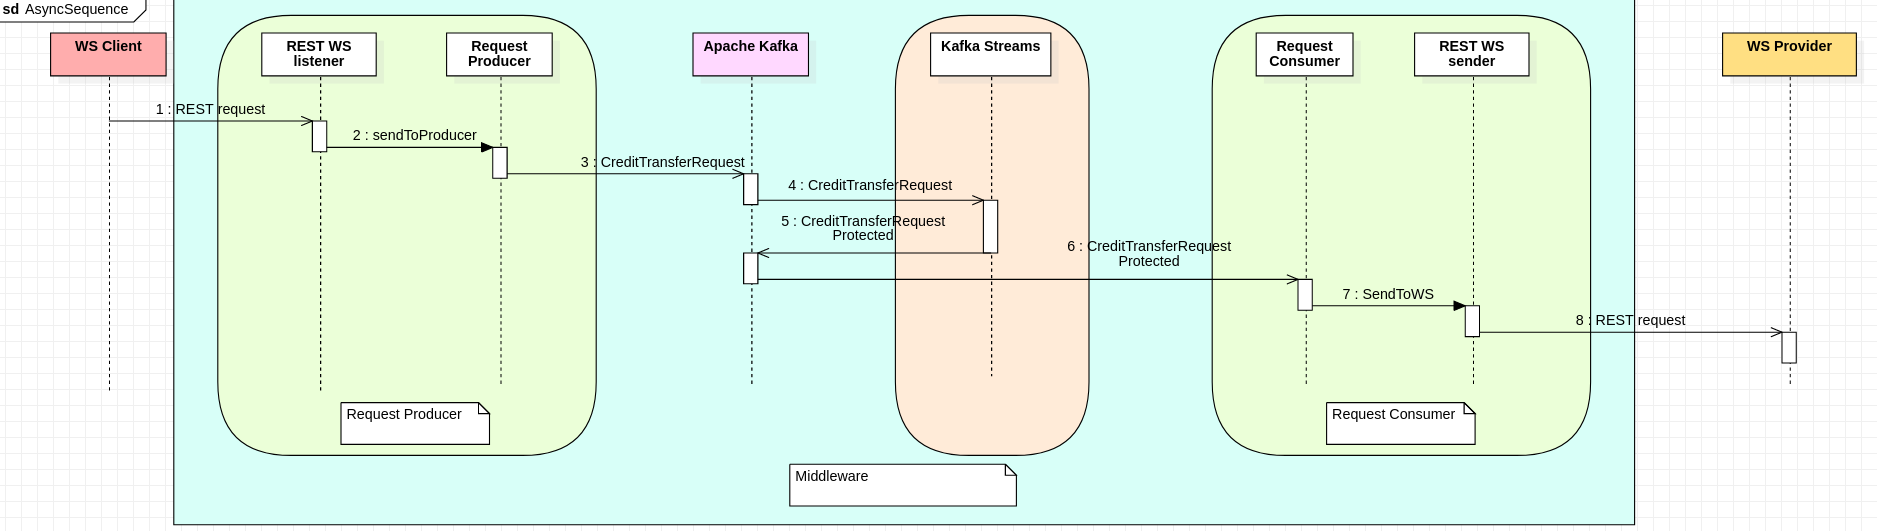
\includegraphics[width=\textwidth]{images/ap_sequence.png}
    \caption{Diagramma di sequenza \sacr{uml} per la reingegnerizzazione del flusso asincrono con protezione dei dati sensibili.}
    \captionsetup{aboveskip=2pt}
    \caption*{\begin{footnotesize}\textit{Fonte: elaborazione personale}\end{footnotesize}}
  \end{center}
\end{figure}

In figura \thefigure\ possiamo vedere il nuovo flusso asincrono con protezione (mascheramento) del dato sensibile.
La versione con \textit{callback} del flusso qui sopra prevede anche il flusso di ritorno (\textit{callback}), non illustrato in figura ma facilmente intuibile grazie al grafico che la precede.

\subsubsection{\sacr{uml} \textit{deployment diagrams}}

A supporto di questi \sacr{uml} \textit{sequence diagram} che rappresentano efficacemente il flusso di dati, punto focale dell'intero sistema di integrazione (asincrono con la protezione del dato sensibile), ho prodotto ulteriori diagrammi, tra i quali il \textit{deployment diagram}.
Questo diagramma ha lo scopo di rappresentare la configurazione dei processi \textit{run time}, modellando la struttura di base in cui eseguono i diversi servizi;
il diagramma esprime l'ambiente in cui i vari componenti risiedono e ove essi comunicano tra di loro.

Con l'approvazione degli esperti aziendali, ho deciso di appoggiare il sistema di integrazione sulla piattaforma Docker.

\begin{figure}[h]
  \begin{center}
    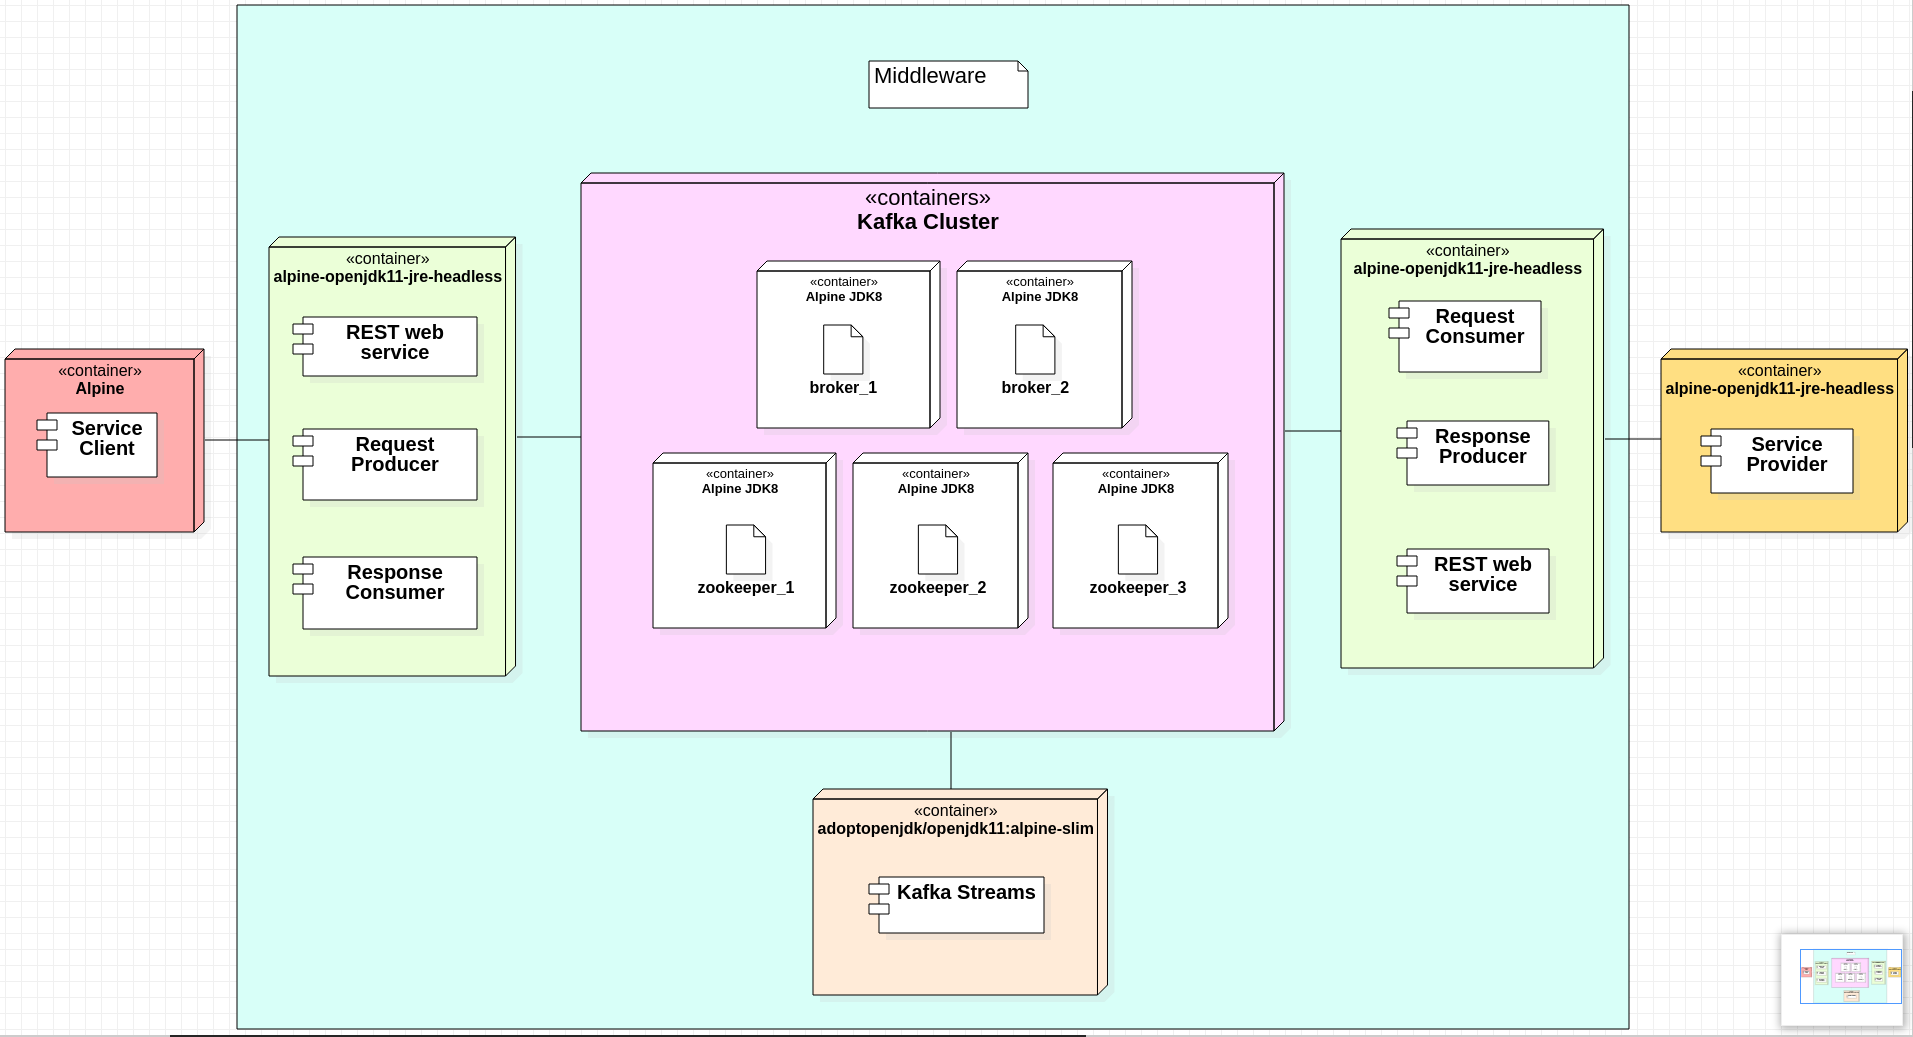
\includegraphics[width=\textwidth,  trim={0 0.2cm 0.2cm 0},clip]{images/ap_deployment.png}
    \caption{\sacr{uml} \textit{deployment diagram} per la reingegnerizzazione del flusso asincrono (protetto)}
    \captionsetup{aboveskip=2pt}
    \caption*{\begin{footnotesize}\textit{Fonte: elaborazione personale}\end{footnotesize}}
  \end{center}
\end{figure}

Il diagramma di \textit{deployment} (figura \thefigure) vede pertanto l'utilizzo di numerosi \textit{container} indipendenti che dialogano attraverso una rete locale all'interno di Docker.
Questi \textit{container} sono raffigurati dai vari nodi (rappresentati dai cubi in rilievo in figura).
A questa notazione fa eccezzione il nodo virtuale intitolato "Kafka Cluster", che ha solamente lo scopo di raggruppare i vari nodi legati al \textit{environment} di Kafka con funzione comune, ma che in realtà non compone un container reale a se stante.
All'interno di questi nodi sono rappresentati gli artefatti che eseguono nel relativo \textit{container}, per esplicitare la presenza dei componenti.
Si può inoltre notare che l'ambiente di Apache Kafka è composto da un \textit{cluster} composto da due servizi \textit{Broker} e tre servizi \textit{Zookeeper}, allo scopo di simulare un caso d'uso reale in cui i diversi componenti sono distribuiti in sistemi indipendenti e garantiscono l'affidabilità dello \textit{streaming} di eventi.

\subsubsection{\sacr{uml} \textit{component diagram}}

\begin{figure}[h]
  \begin{center}
    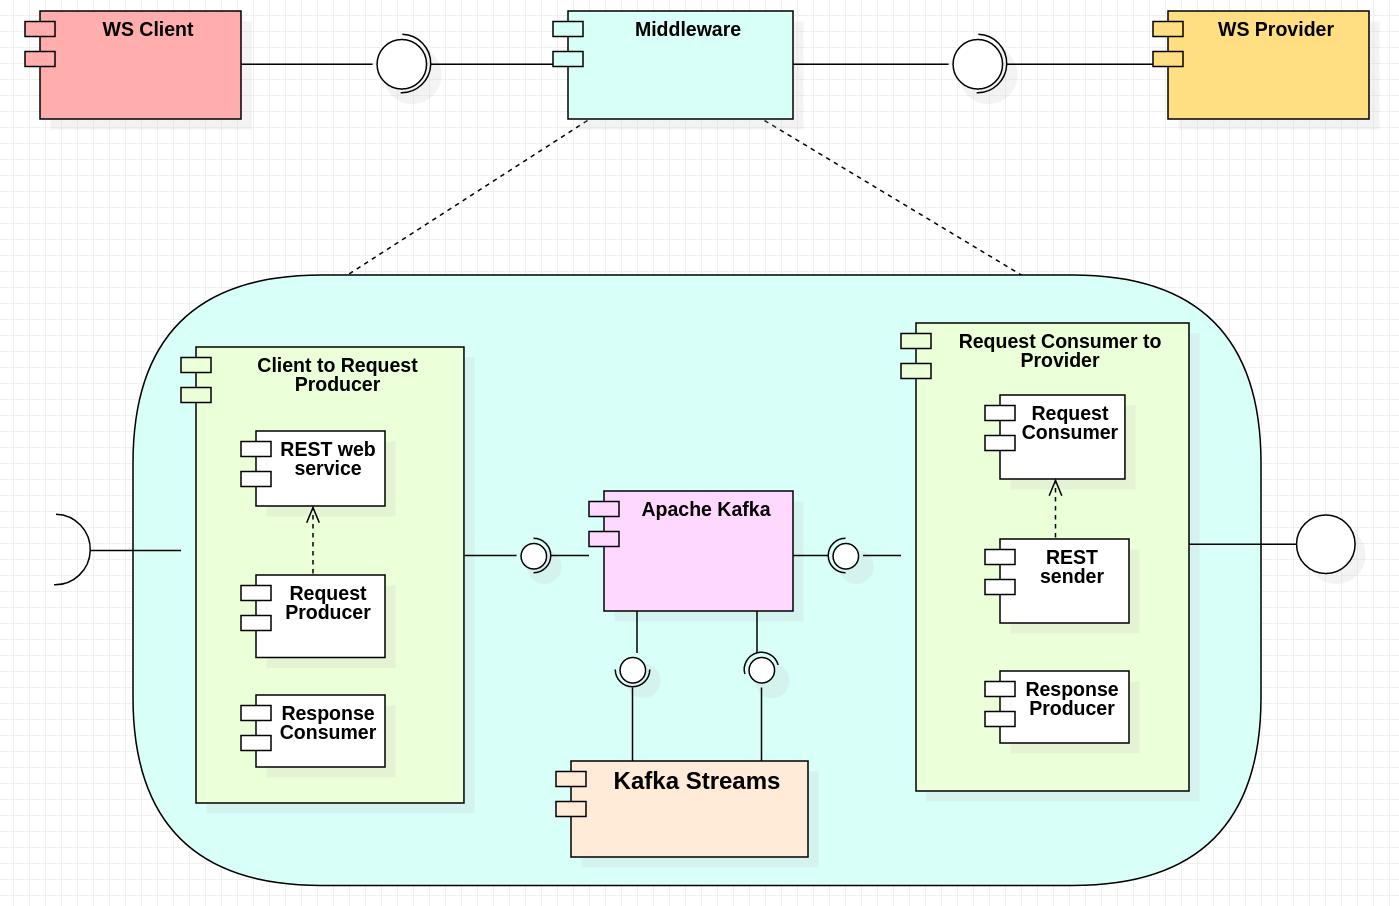
\includegraphics[width=\textwidth]{images/ap_component.png}
    \caption{\sacr{uml} \textit{component diagram} per la reingegnerizzazione del flusso asincrono (protetto)}
    \captionsetup{aboveskip=2pt}
    \caption*{\begin{footnotesize}\textit{Fonte: elaborazione personale}\end{footnotesize}}
  \end{center}
\end{figure}

Allo scopo di riassumere elegantemente i vari componenti del sistema ho elaborato un \sacr{uml} \textit{component diagram}.


% , basati su delle immagini Linux leggere e personalizzate.

% Come si può vedere dalla figura \thefigure,

\section{\textit{Setup} dell'ambiente di lavoro}


\section{Sviluppo}


\section{Collaudo}

Confronto con i requisiti posti nel piano di lavoro, valutazione riguardo i risultati raggiunti, quelli non raggiunti e i possibili sviluppi futuri
